% -------------------------------------------------------------------------------
% Establish page structure & font.
\documentclass[12pt]{report}

\usepackage[total={6.5in, 9in},
	left=1in,
	right=1in,
	top=1in,
	bottom=1in,]{geometry} % Page structure

\usepackage{graphicx} % Required for inserting images
\graphicspath{{../.images/}} % Any additional images I use (BCU logo, etc) are from here.

\usepackage[utf8]{inputenc} % UTF-8 encoding
\usepackage[T1]{fontenc} % T1 font
\usepackage{float}  % Allows for floats to be positioned using [H], which correctly
                    % positions them relative to their location within my LaTeX code.
\usepackage{subcaption}
\usepackage{csquotes}

% -------------------------------------------------------------------------------
% Declare biblatex with custom Harvard BCU styling for referencing.
\usepackage[
    useprefix=true,
    maxcitenames=3,
    maxbibnames=99,
    style=authoryear,
    dashed=false, 
    natbib=true,
    url=false,
    backend=biber
]{biblatex}

\usepackage[british]{babel}

% Additional styling options to ensure Harvard referencing format.
\renewbibmacro*{volume+number+eid}{
    \printfield{volume}
    \setunit*{\addnbspace}
    \printfield{number}
    \setunit{\addcomma\space}
    \printfield{eid}}
\DeclareFieldFormat[article]{number}{\mkbibparens{#1}}

\addbibresource{Report.bib}

% -------------------------------------------------------------------------------
% To prevent "Chapter N" display for each chapter
\usepackage[compact]{titlesec}
\usepackage{wasysym}
\usepackage{import}

\titlespacing*{\chapter}{0pt}{-2cm}{0.5cm}
\titleformat{\chapter}[display]
{\normalfont\bfseries}{}{0pt}{\Huge}

% -------------------------------------------------------------------------------
% Custom macro to make an un-numbered footnote.

\newcommand\blfootnote[1]{
    \begingroup
    \renewcommand\thefootnote{}\footnote{#1}
    \addtocounter{footnote}{-1}
    \endgroup
}

% -------------------------------------------------------------------------------
% Fancy headers; used to show my name, BCU logo and current chapter for the page.
\usepackage{fancyhdr}
\usepackage{calc}
\pagestyle{fancy}

\setlength\headheight{37pt} % Set custom header height to fit the image.

\renewcommand{\chaptermark}[1]{%
    \markboth{#1}{}} % Include chapter name.


% Lewis Higgins - ID 22133848           [BCU LOGO]                [CHAPTER NAME]
\lhead{Lewis Higgins - ID 22133848~~~~~~~~~~~~~~~
\includegraphics[width=1.75cm]{BCU}}
\fancyhead[R]{\leftmark}

% ------------------------------------------------------------------------------
% Used to add PDF hyperlinks for figures and the contents page.

\usepackage{hyperref}

\hypersetup{
    colorlinks=true,
    linkcolor=black,
    filecolor=magenta,
    urlcolor=blue,
    citecolor=black,
}

% ------------------------------------------------------------------------------
\usepackage{xcolor} 
\usepackage{colortbl}
\usepackage{longtable}
\usepackage{amssymb}
% ------------------------------------------------------------------------------
\usepackage{tcolorbox}
\newcommand{\para}{\vspace{7pt}\noindent}
% -------------------------------------------------------------------------------

\title{IOThings Application Report}
\author{Lewis Higgins - Student ID 22133848}
\date{May 2025}

% -------------------------------------------------------------------------------

\begin{document}


\makeatletter
\begin{titlepage}
    \begin{center}
        
\includegraphics[width=0.7\linewidth]{BCU}\\[4ex]
        {\huge \bfseries CMP6207 - Assignment 1}\\[2ex]
        {\large \bfseries  \@title}\\[50ex]
        {\@author}\\[2ex]
        {CMP6207 - Modern Data Stores}\\[2ex]
        {Module Coordinator: Konstantinos Vlachos}\\[5ex]
    \end{center}
\end{titlepage}
\makeatother
\thispagestyle{empty}
\newpage


% Page counter trick so that the contents page doesn't increment it.
\setcounter{page}{0}

\tableofcontents
\thispagestyle{empty}

\chapter*{Introduction}
\addcontentsline{toc}{chapter}{Introduction}
The report will be based on the design and implementation of a MongoDB NoSQL database system 
for the company "IoThings Home Automation Solutions". There are two assignments in this module, where this report is
worth \textbf{60\%}, and a presentation is the remaining \textbf{40\%}. This module 
will also incorporate elements of web design, with HTML and CSS also playing a role alongside the primary 
use of JavaScript.

\begin{itemize}
    \item Konstas cares more for the functionality over aesthetics. While you should put effort into 
    the HTML and CSS parts, they're a lesser concern than the overall usability of the system.
    \item A literature review is expected in this report.
    \item 4,000 word count, so 4,400 hard limit.
    \item The presentation is about this report. It must cover the design, implementation and data management.
    \begin{itemize}
        \item You would show him your database cluster (local or Atlas?) as part of it.
    \end{itemize}
    \item IT WILL BE THIRTY MINUTES. If the report contains all the screenshots (which it will) you might not need 
    to make slides, though consider it anyway. You can still show the report alongside the slides where needed.
    \item He wants you to make an Atlas account even if you do it locally.
    \item You are creating the dataset for this assignment. You will describe it in an appendix rather than 
    the report's main body.
    \item This is a "professional report", and as such the title page with the BCU logo and your info should 
    probably change. It needs to also show the date.
\end{itemize}

\chapter{Types of NoSQL databases}

\noindent Structured Query Language, or SQL, was developed by IBM following \textcite{codd_relational_1970}'s groundbreaking 
publication in the ACM journal, with the first commercial SQL implementation being published by Oracle in 1979 \autocite{oracle_history_nodate}.
SQL powers many relational database systems even today, though the problems associated with its age, most notably in 
the speed of its operations, are beginning to show in modern systems. Therefore, NoSQL ("Not Only SQL") was developed as 
an extension of SQL, allowing data to be stored in a non-tabular, non-relational format for efficient storage of
semi-structured and unstructured data in a flexible, functional and scalable model for faster operations than standard 
relational databases in most scenarios \autocite{google_cloud_what_nodate, aws_what_nodate}. There are a wide variety of NoSQL 
database types which vary in complexity, functionality and purpose, meaning that identification of the most suitable type is paramount 
for maximum efficiency. 

\section{Document database}
% ? MongoDB is a document database.
% * General purpose databases.
Document databases are intuitive, flexible and horizontally scalable databases that work well in a wide variety of general purpose use cases.
They store records as "documents", which store an object's data and metadata, in a format such as JSON
\footnote{JavaScript Object Notation}, BSON \footnote{Binary JSON}, or XML \footnote{Extensible Markup Language}. 

\begin{figure}[H]
    \centering
    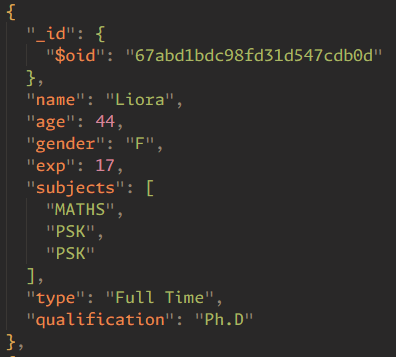
\includegraphics[width=0.5\textwidth]{NoSQL DBs/Doc/ExampleDoc}
    \caption{An example of a JSON Document.\label{fig:ExampleDoc}}
\end{figure}

\noindent Figure \ref{fig:ExampleDoc} depicts an example JSON document of a school teacher stored in MongoDB, a popular DBMS
for document databases. Within it, the internal object ID (metadata) is stored, as well as other data of varying types including 
strings, integers and arrays. This makes document databases easily integratable into a development workflow due to the direct 
storage of object types typically used in programming languages like Python and JavaScript.




\section{Key-value database}
% * Very fast, very simple.

\section{Column-oriented database}
% * Stores data in columns rather than rows.
% * Fast reading, slow writing. 
% * Better for OLAP than OLTP iirc.
% ! In the scenario, the slow writing means it's unwanted. Client wants IoT sensor data recorded, so it'll be lots of writing.


\section{Graph database}
% ? Neo4J is a graph database.


\section{In-memory database}
% ? Redis is an in-memory database.
% ! While that's true, it's also a key-value database.


\chapter{Comparing NoSQL and Relational databases} 
% ! Chapter title doesn't fit the page.
\begin{itemize}
    \item Compare types of NoSQL databases here.
    \item This section "shouldn't be too long, but enough to convince them."
    \item \textbf{This is NOT comparing \textit{MongoDB} to relational databases.} The brief 
    mentions that it should be "generic just in case after seeing your MongoDB database
    they decide to go with another software provider."
\end{itemize}
  

% Assuming this is probably the longest chapter.
\chapter{Database design and implementation}

MongoDB, an acronym from "hu\textbf{mongo}us \textbf{DB}", aims to address some of SQL's antiquation issues\dots
% ! I want to be up to this point by Feb 28th.

\chapter{API Implementation and Documentation}


\chapter*{Conclusion}
\addcontentsline{toc}{chapter}{Conclusion}
% ! I want to be done with this report by April 14th, with the 
% ! April 29 - May 4 window being for final improvements and presentation prep.

Overall, something was done\dots



\printbibliography
\addcontentsline{toc}{chapter}{Bibliography}



\end{document}